\chapter{Planificación}

\section{Planificación}

En esta sección se presenta un diagrama de Gantt que recoge la planificación temporal del proyecto, abarcando los meses de marzo a agosto. El diagrama refleja las principales tareas a realizar, correspondientes a los siete objetivos específicos expuestos previamente, y permite visualizar la distribución y el solapamiento de actividades a lo largo de todo el desarrollo.

\begin{figure}[H]
    \centering
    \fbox{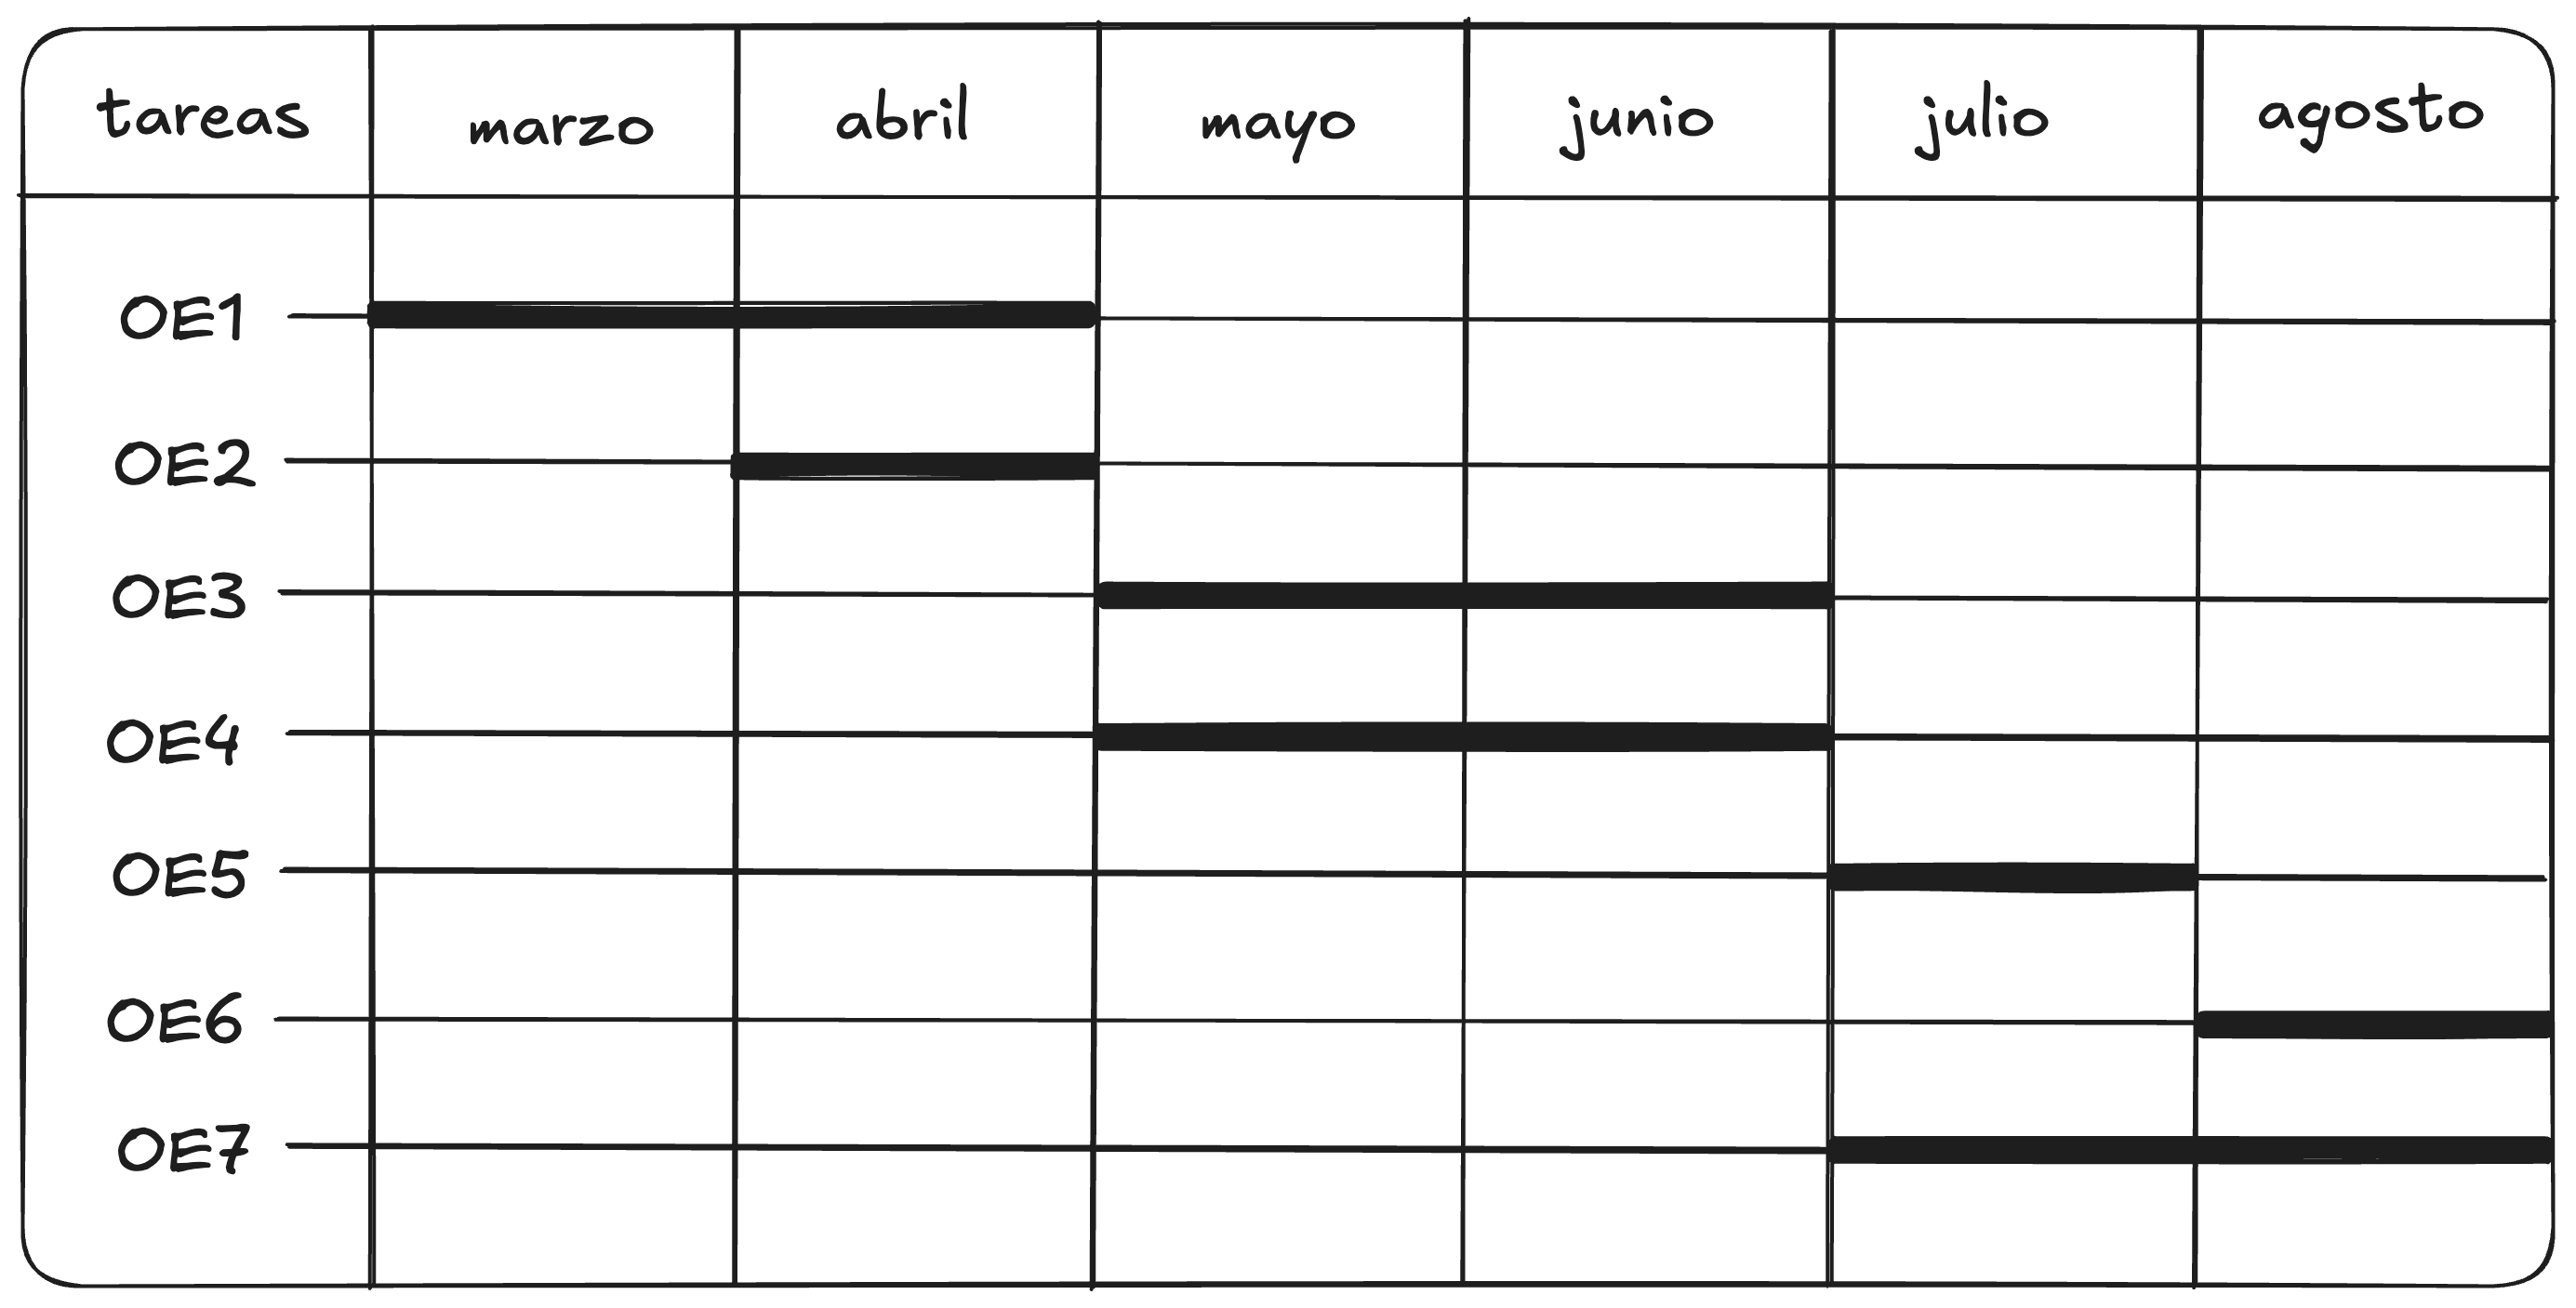
\includegraphics[width=\textwidth]{imagenes/gantt1.png}}
    %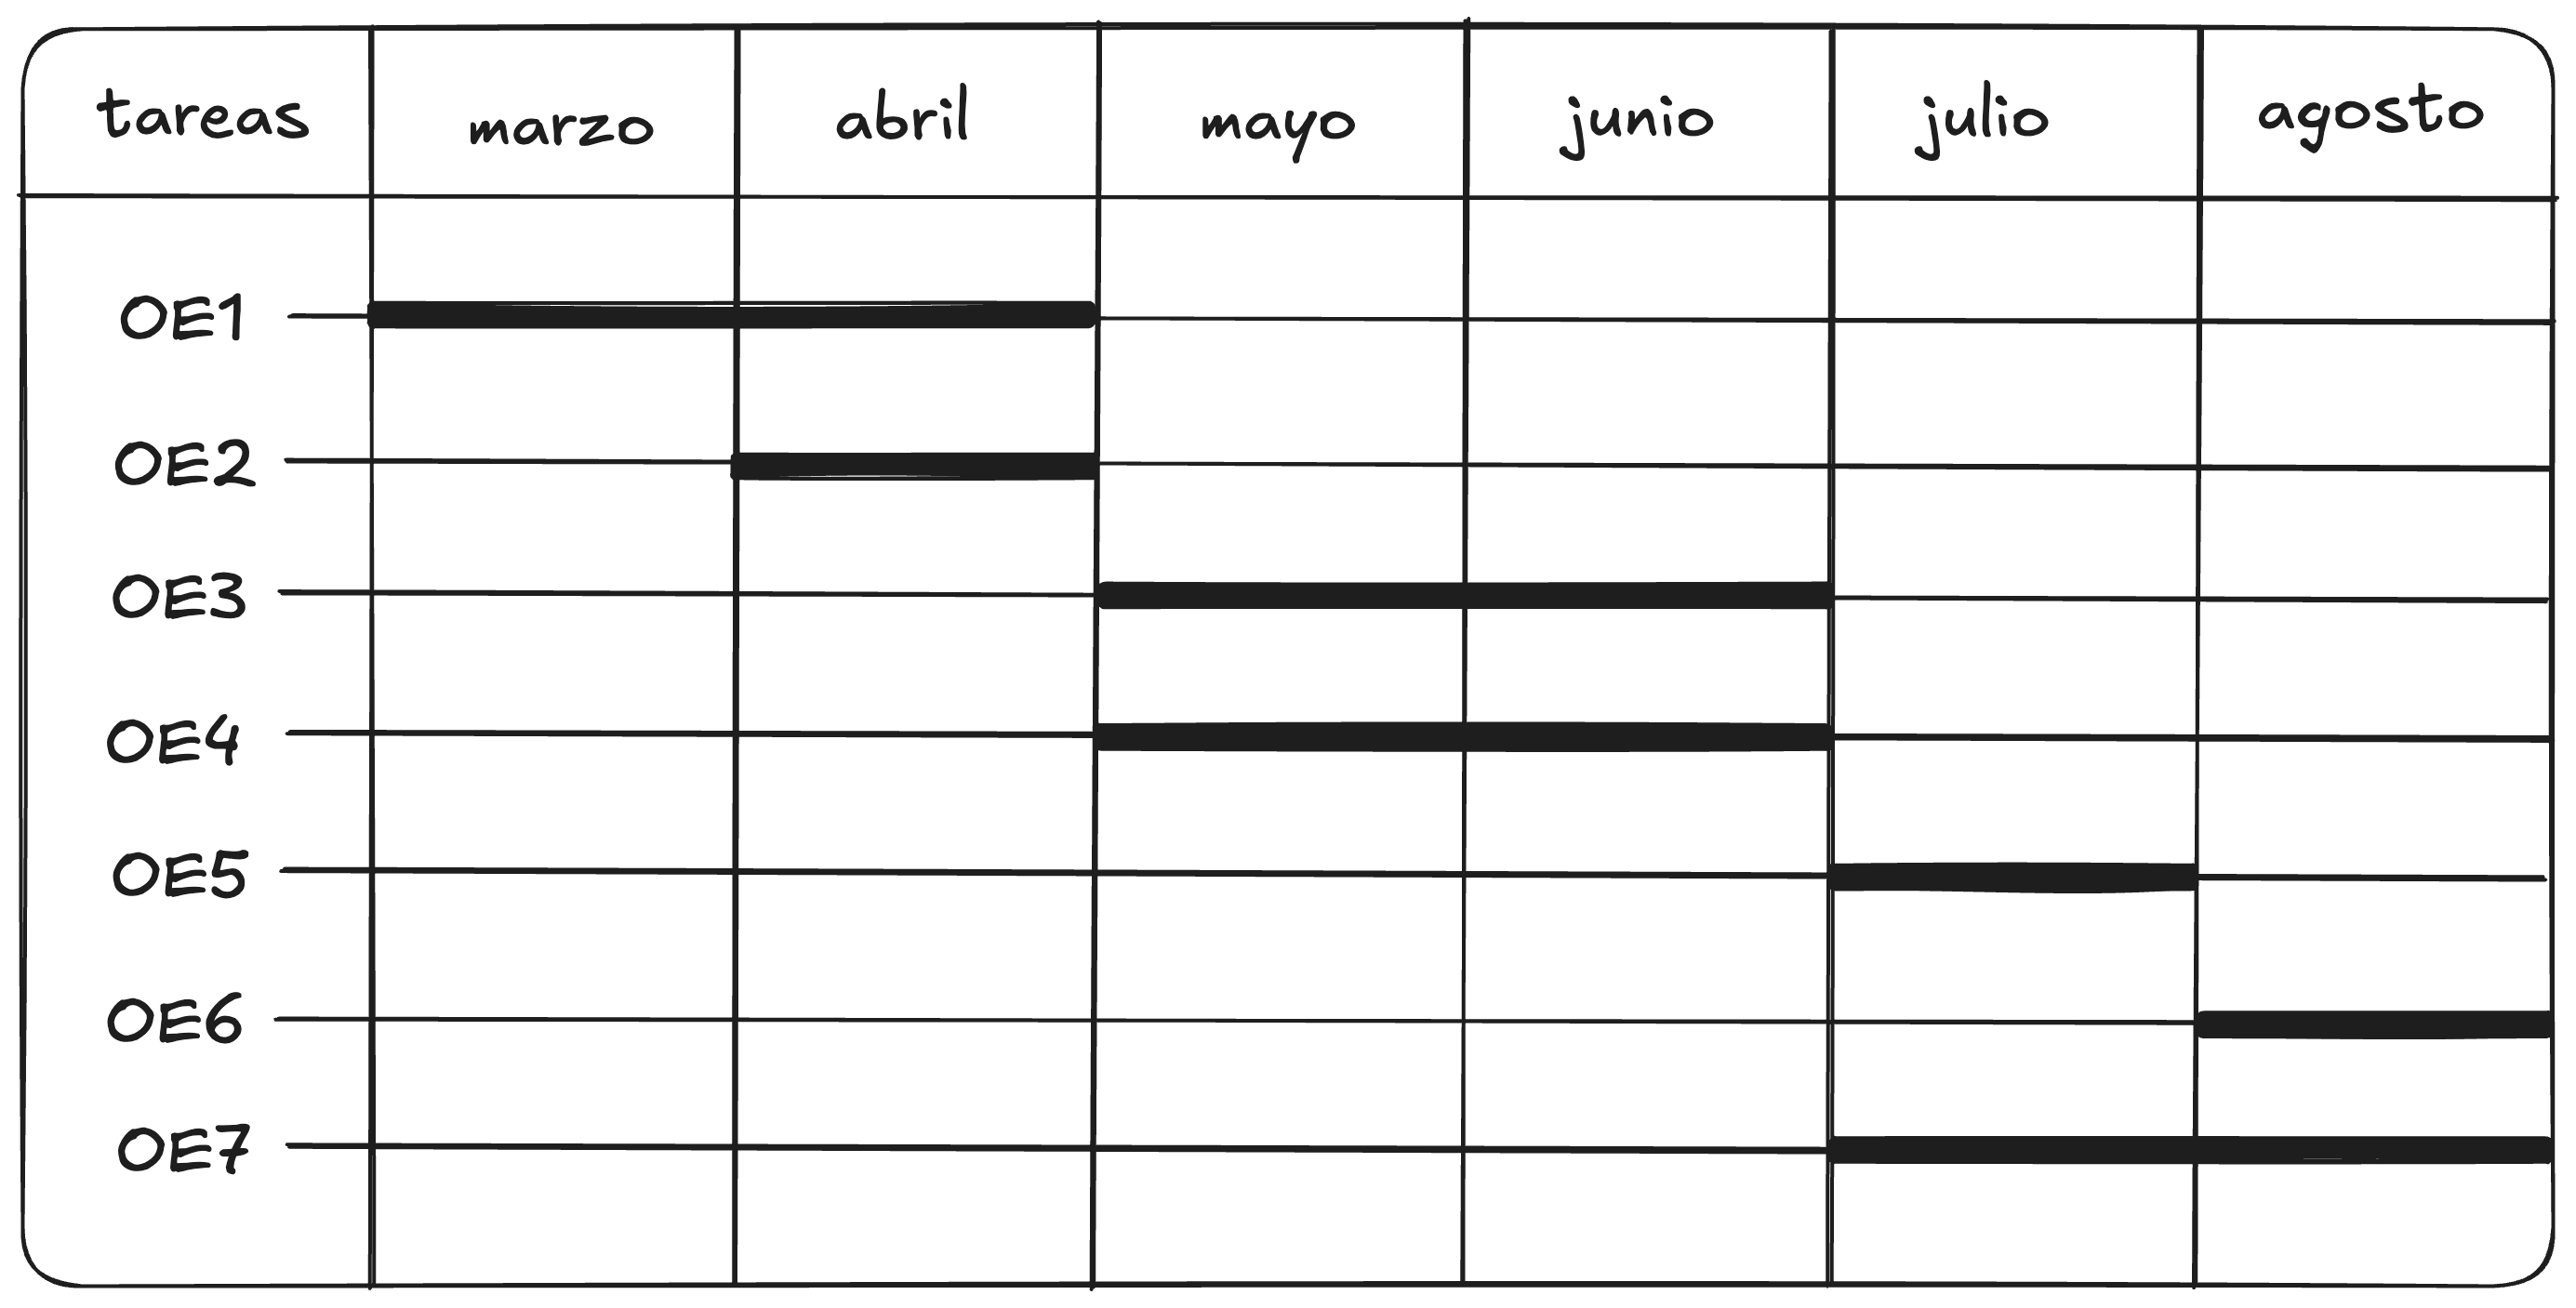
\includegraphics[width=\textwidth]{imagenes/gantt1.png}
    \caption{Diagrama de Gantt con la planificación del proyecto.}
\end{figure}

\section{Costes}

Si bien este proyecto tiene un enfoque académico, la elaboración de un presupuesto permite obtener una perspectiva más objetiva sobre el trabajo realizado. Este ejercicio aporta tanto un marco técnico como económico, acercando la iniciativa a escenarios reales y facilitando estimaciones útiles para futuras implementaciones o propuestas. Asimismo, contribuye a fundamentar las decisiones técnicas en función de su viabilidad financiera.

Para la estimación de costes, se han tenido en cuenta los recursos humanos, el equipamiento tecnológico y las herramientas de software empleadas. El cálculo se apoya en las tarifas promedio del sector de la programación en España y en los recursos técnicos requeridos. Los datos salariales se han extraído de la plataforma Glassdoor \cite{glassdoor}. Se ha considerado una duración total del proyecto de cinco meses.

\subsubsection{Costes humanos}

Para simular el coste de desarrollo de la plataforma en un entorno real, se ha considerado la contratación de un desarrollador junior a jornada completa (8 horas diarias, 21 días laborables al mes), lo que supone 168 horas mensuales. El salario anual medio para este perfil en España se estima en 20.000€.

\begin{equation*}
\text{Horas trabajadas al año} = 168\,\text{horas/mes} \times 12\,\text{meses} = 2.016\,\text{horas/año}
\end{equation*}

\begin{equation*}
\text{Coste por hora} = \frac{20.000\,€}{2.016\,\text{horas}} \approx 9,92\,€/hora
\end{equation*}

\begin{equation*}
\text{Coste mensual} = 9,92\,€/hora \times 168\,\text{horas} = 1.666,56\,€
\end{equation*}

\begin{equation*}
\text{Coste total (5 meses)} = 1.666,56\,€ \times 5 = 8.332,80\,€
\end{equation*}

\subsubsection{Costes de material}

Para el desarrollo del proyecto se han utilizado los siguientes equipos. Dado que el hardware tiene una vida útil superior a la duración del proyecto, se ha calculado el coste imputable en función del tiempo de uso exclusivo para este trabajo (5 meses, aproximadamente 0,42 años):

\begin{center}
\begin{tabular}{|l|c|c|c|}
\hline
\textbf{Material} & \textbf{Precio compra (€)} & \textbf{Vida útil (años)} & \textbf{Coste imputable (€)} \\
\hline
Ordenador portátil & 2.000 & 4 & 210,00 \\
Servidor doméstico & 500 & 5 & 42,00 \\
\hline
\multicolumn{3}{|r|}{\textbf{Total}} & \textbf{252,00} \\
\hline
\end{tabular}
\end{center}

\noindent El cálculo del coste imputable sigue la fórmula:
\begin{equation*}
\text{Coste imputable} = \frac{\text{Precio de compra}}{\text{Vida útil (años)}} \times \text{Tiempo de uso (años)}
\end{equation*}

\subsubsection{Costes de herramientas}

Todo el software empleado en el desarrollo del proyecto corresponde a herramientas de licencia gratuita o planes gratuitos, por lo que no suponen coste adicional. No obstante, se ha utilizado la API de OpenAI con un coste total de 20€, además de un dominio personalizado con coste de 10€.

\begin{center}
\begin{tabular}{|l|c|}
\hline
\textbf{Herramienta} & \textbf{Coste (€)} \\
\hline
Software (licencias gratuitas) & 0 \\
Dominio & 10 \\
API OpenAI & 20 \\
\hline
\textbf{Total} & \textbf{30} \\
\hline
\end{tabular}
\end{center}

\subsubsection{Resumen de costes}

A continuación se muestra un resumen de todos los costes estimados para el proyecto:

\begin{center}
\begin{tabular}{|l|c|}
\hline
\textbf{Concepto} & \textbf{Coste (€)} \\
\hline
Coste de personal & 8.332,80 \\
Coste de material & 252,00 \\
Coste de herramientas & 30 \\
\hline
\textbf{Total} & \textbf{8.614,80} \\
\hline
\end{tabular}
\end{center}